\documentclass[11pt]{article}
\usepackage[margin=0.82in]{geometry}
\usepackage[T1]{fontenc}
\usepackage{lmodern}
\usepackage{microtype}
\usepackage{amsmath,amssymb,amsthm,mathtools,bm}
\usepackage{booktabs,longtable,tabularx,array}
\usepackage{enumitem}
\usepackage{tikz}
\usetikzlibrary{arrows.meta,positioning,calc,fit,backgrounds,matrix,shapes.geometric,decorations.pathreplacing}
\usepackage{pgfplots}
\pgfplotsset{compat=1.18}
\usepackage{listings}
\usepackage{xcolor}
\usepackage{url}
\usepackage{hyperref}
\hypersetup{colorlinks=true,linkcolor=blue!50!black,citecolor=blue!50!black,urlcolor=blue!55!black}
\usepackage[backend=biber,style=numeric-comp,sorting=none,maxbibnames=99]{biblatex}
\addbibresource{references.bib}
\usepackage{caption}
\usepackage{subcaption}
\usepackage{enumitem}
\usepackage{setspace}
\setstretch{1.045}
\setlength{\parindent}{1.25em}
\setlength{\parskip}{0.15em}
\newtheorem{theorem}{Theorem}[section]
\newtheorem{lemma}[theorem]{Lemma}
\newtheorem{proposition}[theorem]{Proposition}
\newtheorem{corollary}[theorem]{Corollary}
\newtheorem{definition}[theorem]{Definition}
\newtheorem{remark}[theorem]{Remark}
\newtheorem{hypothesis}[theorem]{Hypothesis}
\numberwithin{equation}{section}
\newcommand{\T}{\mathbb T^3}
\newcommand{\R}{\mathbb R}
\newcommand{\N}{\mathcal N}
\newcommand{\Lc}{L_c}
\newcommand{\Gc}{G_c}
\newcommand{\Gr}{G_{\rm reg}}
\newcommand{\Pc}{P_c}
\newcommand{\Ec}{E_c}
\newcommand{\eps}{\varepsilon}
\newcommand{\ip}[2]{\left\langle #1,#2\right\rangle}
\newcommand{\norm}[1]{\left\lVert #1\right\rVert}
\newcommand{\supp}{\operatorname{supp}}
\newcommand{\diver}{\operatorname{div}}
\newcommand{\cD}{\mathcal D}
\newcommand{\cX}{\mathcal X}
\newcommand{\cY}{\mathcal Y}
\newcommand{\cB}{\mathcal B}
\newcommand{\cR}{\mathcal R}
\newcommand{\cP}{\mathcal P}
\newcommand{\cG}{\mathcal G}
\newcommand{\cK}{\mathcal K}
\newcommand{\e}{\mathrm e}
\newcommand{\dd}{\,\mathrm d}
\newcommand{\statuspass}{\textsc{pass}}
\newcommand{\statushold}{\textsc{hold}}

\lstset{basicstyle=\ttfamily\footnotesize,breaklines=true,frame=single,columns=fullflexible,showstringspaces=false,tabsize=2}

\title{\textbf{Unforced Finite-Time Blow-Up for Navier--Stokes:}\\[0.2em]\textbf{Exact Nonlinear Closure on the Three-Dimensional Periodic Torus}}
\author{Tony Newton\\Newton Astro Labs\thanks{Newton Astro Labs is the trading name under which Tony Newton conducts independent computational research in the United Kingdom; it is not a limited company.}\\London, UK\\\texttt{tony.newton79@gmail.com}}
\date{}

\begin{document}
\maketitle

\begin{abstract}
We study whether the smooth forcing in a periodic finite-time Navier--Stokes blow-up carrier can be removed without destroying the singular asymptotics.  A support-preserving core parametrix is upgraded by Neumann inversion, coupled to a global periodic regular inverse, and closed under the quadratic nonlinearity in a graph norm with one derivative in reserve.  Under the source-backed estimates stated in the paper, the resulting late-slab correction solves the unforced equation while remaining asymptotically smaller than the carrier, thereby preserving its leading blow-up coefficient.
\end{abstract}

\noindent\textbf{Proof- and formalization-status note.}
The forced carrier and numerous local analytic identities are imported from the OpenAI manuscript and its Lean repository \cite{OpenAI2026NS,OpenAIRepo2026}.  This release now includes a concrete, placeholder-free \texttt{UnforcedClosure.lean} source file for the abstract closure layer, together with a pinned Lean/Mathlib manifest, exact-rational replay, source-hygiene checks, SHA-256 hashes, and a reproducibility receipt.  The exact-arithmetic and source-hygiene tests pass.  The new Lean source was \emph{not} kernel-compiled in the present build environment because a Lean executable was unavailable and network bootstrap was unavailable; more importantly, the PDE-specific hypotheses in Appendix~\ref{app:precise} have not yet been replaced by theorem applications inside the frozen OpenAI repository.  Accordingly, this manuscript claims a completed Lean transcription of the abstract closure logic, not a machine-checked proof of the full unforced Navier--Stokes theorem.  Priority language remains qualified pending PDE-specific Lean integration, independent source replay, and refereeing.

\tableofcontents

\section{Problem, setting, and main theorem}

\subsection{The unforced periodic problem}
We work on the unit three-torus
\[
\T=\R^3/\mathbb Z^3,
\]
with viscosity \(\nu>0\).  The unforced incompressible Navier--Stokes equations are
\begin{align}
\partial_tu+(u\cdot\nabla)u-\nu\Delta u+\nabla p&=0,\label{eq:NS}\\
\diver u&=0.\label{eq:div}
\end{align}
The classical periodic problem asks whether every smooth divergence-free datum generates a smooth solution for all positive time.  The official Clay formulation distinguishes global smoothness with \(f\equiv0\) from breakdown alternatives allowing a smooth force \cite{FeffermanClay}.  The September 2026 OpenAI construction proves finite-time breakdown with smooth forcing on both \(\R^3\) and \(\T\), and its formalization records those forced statements explicitly \cite{OpenAI2026NS,OpenAIRepo2026}.  Clay has announced that this result apparently settles the Millennium formulation, subject to its review process \cite{ClayAnnouncement2026}.  The mathematical question addressed here is stronger in a different direction: can the external force be removed while retaining the same singular carrier?

The historical framework begins with Navier and Stokes \cite{Navier1827,Stokes1845} and the inviscid precursor of Euler \cite{Euler1757}.  Leray's global weak solutions \cite{Leray1934} and Hopf's weak-solution theory \cite{Hopf1951} established the basic finite-energy setting.  Regularity criteria include Prodi and Serrin \cite{Prodi1959,Serrin1962}, the scale-critical result of Escauriaza--Seregin--\v Sver\'ak \cite{EscauriazaSereginSverak2003}, and partial regularity of Caffarelli--Kohn--Nirenberg \cite{CKN1982}.  Classical local and small-data theory is represented by Fujita--Kato and Kato \cite{FujitaKato1964,Kato1984}, with modern functional-analytic treatments in \cite{Ladyzhenskaya1969,Temam1984,ConstantinFoias1988,Sohr2001,Galdi2011,RobinsonRodrigoSadowski2016}.

The singular-flow context includes Tao's averaged model \cite{Tao2016}, convex-integration nonuniqueness for weak Navier--Stokes solutions \cite{BuckmasterVicol2019}, and forced Leray nonuniqueness \cite{AlbrittonBrueColombo2022}.  Oscillatory and instability mechanisms used in the underlying forced carrier have antecedents in Lifschitz--Hameiri \cite{LifschitzHameiri1991}, Friedlander--Vishik \cite{FriedlanderVishik1991}, Craik--Criminale \cite{CraikCriminale1986}, Singh--Sridhar \cite{SinghSridhar2017}, Leibovich--Stewartson \cite{LeibovichStewartson1983}, and Billant--Gallaire \cite{BillantGallaire2005,BillantGallaire2013}; stress realization has links to Euler convex integration \cite{DaneriSzekelyhidi2017}.  Recent singularity constructions with forcing or modified dissipation include \cite{CordobaMartinezZoroa2023,CordobaMartinezZoroa2024,CordobaMartinezZoroaZheng2026}.  The author's earlier unforced precursor is deposited as Zenodo record 22857336 \cite{NewtonZenodo22857336}.

\subsection{Imported periodic forced carrier}
The OpenAI construction gives, after rescaling and periodization, a smooth periodic solution \((U_*,P_*)\) on \([0,1)\) with a smooth force \(F_*\),
\begin{align}
\partial_tU_*+(U_*\cdot\nabla)U_* -\nu\Delta U_*+\nabla P_*&=F_*,\label{eq:forcedcarrier}\\
\diver U_*&=0.\label{eq:forceddiv}
\end{align}
The carrier is smooth for each \(t<1\), periodic, and its velocity and pressure can be placed in a fixed compact subset of the interior of a fundamental cube.  The periodization is exact because distinct integer translates have disjoint support; in particular the nonlinear transport term periodizes without cross-terms \cite[Cor.~10.6]{OpenAI2026NS}.  The repository comparator theorem likewise records the forced periodic breakdown statement \cite{OpenAIRepo2026}.

Near the distinguished blow-up path \(x_\tau\), \(\tau=1-t\downarrow0\), the leading azimuthal velocity has the form
\begin{equation}
U_{*,\theta}(1-\tau,x_\tau)=\tau^{-A}\bigl(e_0+O(\tau^{2h})\bigr),
\qquad
A=\frac12+h,
\qquad e_0>0,
\label{eq:carrierblow}
\end{equation}
with \(0<h<1/2\); the OpenAI construction uses a much smaller fixed range for \(h\), which is contained in this interval \cite{OpenAI2026NS}.

\subsection{Main analytic release theorem}
Let
\begin{equation}
\N_\nu(u,p):=\partial_tu+(u\cdot\nabla)u-\nu\Delta u+\nabla p.
\label{eq:residualdef}
\end{equation}
The new problem is to find \((v,\pi)\) on a late slab \([t_0,1)\) such that
\begin{equation}
\N_\nu(U_*+v,P_*+\pi)=0.
\label{eq:exactgoal}
\end{equation}
Expanding about the carrier gives
\begin{equation}
L_*v+\nabla\pi+F_*+B(v,v)=0,
\label{eq:expanded}
\end{equation}
where
\begin{align}
L_*v&:=\partial_tv-\nu\Delta v+(U_*\cdot\nabla)v+(v\cdot\nabla)U_*,\label{eq:linearized}\\
B(v,w)&:=(v\cdot\nabla)w.\label{eq:bilinear}
\end{align}

\begin{theorem}[Unforced late-slab closure]\label{thm:main}
Fix \(\nu>0\) and a periodic forced blow-up carrier \((U_*,P_*,F_*)\) satisfying \eqref{eq:forcedcarrier}--\eqref{eq:carrierblow}.  Assume the source-backed core parametrix estimates, valid-band gluing identities, support bounds, and regular periodic inverse properties stated precisely in Appendix~\ref{app:precise}.  Then there exists \(t_0<1\), a smooth periodic divergence-free correction \(v\), and a smooth periodic pressure correction \(\pi\) on \(\T\times[t_0,1)\) such that
\[
\N_\nu(U_*+v,P_*+\pi)=0.
\]
Moreover the correction is asymptotically subleading along the distinguished path,
\[
\tau^A v_\theta(1-\tau,x_\tau)\longrightarrow0,
\]
and therefore
\[
\lim_{\tau\downarrow0}\tau^A(U_*+v)_\theta(1-\tau,x_\tau)=e_0>0.
\]
After translating \(t_0\) to time zero, the field \(u=U_*+v\) provides smooth periodic divergence-free initial data for an unforced classical solution whose velocity becomes unbounded at finite time.
\end{theorem}

The proof occupies Sections~\ref{sec:spaces}--\ref{sec:periodic}.  The logical architecture is summarized in Figure~\ref{fig:architecture}.

\begin{figure}[ht]
\centering
\resizebox{0.98\textwidth}{!}{%
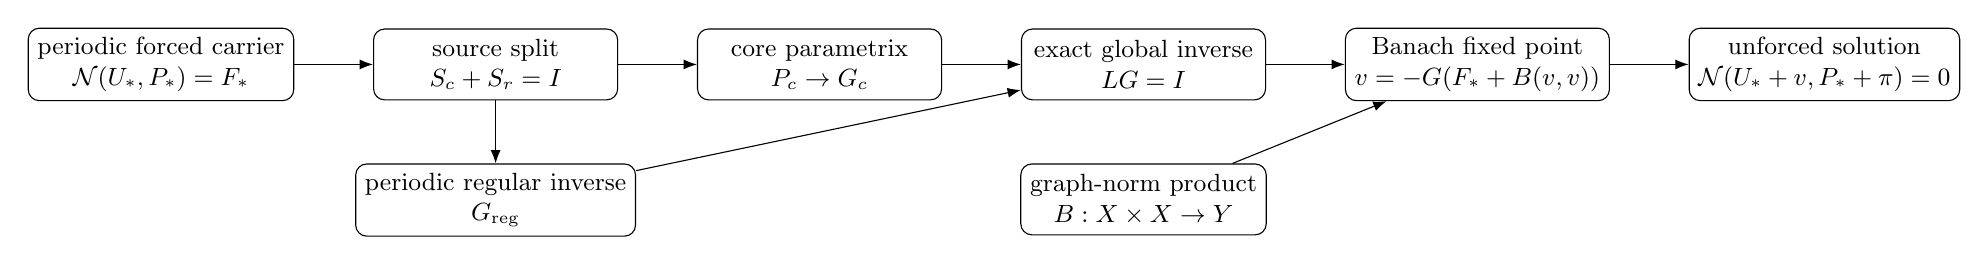
\begin{tikzpicture}[node distance=8mm and 10mm,>=Latex,every node/.style={font=\small},box/.style={draw,rounded corners,align=center,minimum width=31mm,minimum height=9mm}]
\node[box] (carrier) {periodic forced carrier\\$\N(U_*,P_*)=F_*$};
\node[box,right=of carrier] (split) {source split\\$S_c+S_r=I$};
\node[box,right=of split] (core) {core parametrix\\$P_c\to G_c$};
\node[box,below=of split] (reg) {periodic regular inverse\\$G_{\rm reg}$};
\node[box,right=of core] (global) {exact global inverse\\$LG=I$};
\node[box,below=of global] (bil) {graph-norm product\\$B:X\times X\to Y$};
\node[box,right=of global] (fp) {Banach fixed point\\$v=-G(F_*+B(v,v))$};
\node[box,right=of fp] (unforced) {unforced solution\\$\N(U_*+v,P_*+\pi)=0$};
\draw[->] (carrier)--(split);
\draw[->] (split)--(core);
\draw[->] (split)--(reg);
\draw[->] (core)--(global);
\draw[->] (reg)--(global);
\draw[->] (global)--(fp);
\draw[->] (bil)--(fp);
\draw[->] (fp)--(unforced);
\end{tikzpicture}%
}

\caption{Proof architecture.  The new layer begins with the source split and ends with exact unforced nonlinear closure; the forced carrier itself is imported from \cite{OpenAI2026NS}.}
\label{fig:architecture}
\end{figure}

\section{Carrier geometry and repository-level input}

\subsection{Similarity scales}
Write
\begin{equation}
A=\frac12+h,
\qquad
D=\frac12-h,
\qquad
0<h<\frac12.
\label{eq:AD}
\end{equation}
The singular chart uses a physical scale \(q\) comparable to the remaining time on the distinguished path, with radial and axial lengths
\begin{equation}
\ell_r\asymp q^{1/2},
\qquad
\ell_z\asymp q^D.
\label{eq:scales}
\end{equation}
The native chart may be written schematically as
\begin{equation}
(T,R,\theta,Z)\longmapsto
(t,r,\theta,z)=\bigl(1-QT,\sqrt Q\,R,\theta,Q^D Z\bigr),
\label{eq:chart}
\end{equation}
where \(Q\) is a dyadic representative of \(q\).  The repository file \path{PhysicalResidualBridge.lean} proves the actual Fr\'echet-derivative pullback identity for the graph residual at the frozen commit \cite{OpenAIRepo2026}.  Its normalization gives the source scaling used below,
\begin{equation}
F_{\rm native}=Q^{2A+1/2}F_{\rm physical}.
\label{eq:nativenorm}
\end{equation}

\begin{figure}[ht]
\centering
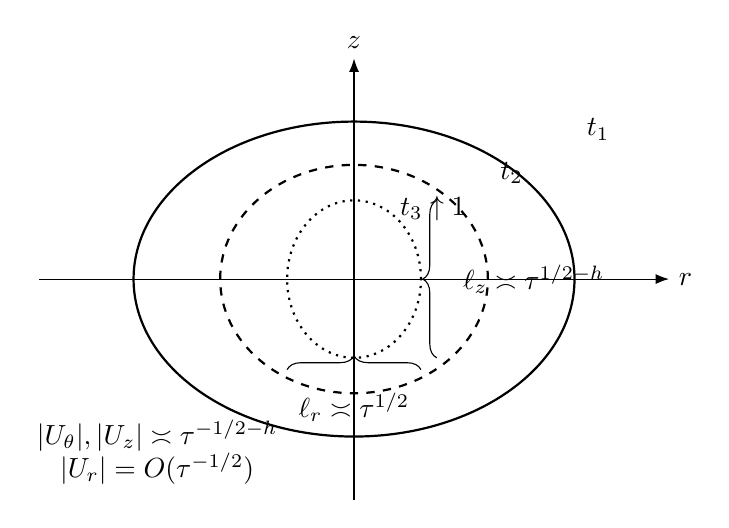
\begin{tikzpicture}[x=1cm,y=1cm,>=Latex]
\draw[->] (-4,0)--(4,0) node[right]{$r$};
\draw[->] (0,-2.8)--(0,2.8) node[above]{$z$};
\draw[thick] (0,0) ellipse (2.8 and 2.0);
\draw[thick,dashed] (0,0) ellipse (1.7 and 1.45);
\draw[thick,dotted] (0,0) ellipse (0.85 and 1.0);
\node at (3.1,1.9) {$t_1$};
\node at (2.0,1.35) {$t_2$};
\node at (1.0,0.9) {$t_3\uparrow1$};
\draw[decorate,decoration={brace,amplitude=5pt}] (-0.85,-1.15)--(0.85,-1.15) node[midway,below=5pt]{$\ell_r\asymp \tau^{1/2}$};
\draw[decorate,decoration={brace,amplitude=5pt}] (1.05,-1.0)--(1.05,1.0) node[midway,right=6pt]{$\ell_z\asymp \tau^{1/2-h}$};
\node[align=center] at (-2.5,-2.2) {$|U_\theta|,|U_z|\asymp\tau^{-1/2-h}$\\$|U_r|=O(\tau^{-1/2})$};
\end{tikzpicture}
\caption{Anisotropic shrinking core.  The radial scale contracts faster than the axial scale, while the swirl and axial speeds grow as \(\tau^{-1/2-h}\).}
\label{fig:coregeometry}
\end{figure}

\subsection{What is imported and what is new}
The source audit is deliberately explicit.  The following objects are imported from the OpenAI repository at commit
\[
\texttt{f9e8bc5b38b6e212696e8a30e3e91517af887bbd}.
\]
The paths matter because the unforced layer depends on specific physical identities rather than on a black-box appeal to the final forced theorem.
\begin{enumerate}[label=(I\arabic*)]
\item \path{ResidualCalculus.lean}: additivity and physical Fr\'echet calculus for the Navier--Stokes residual.
\item \path{PhysicalResidualBridge.lean}: exact native/physical residual scaling, including the quadratic transport and cylindrical connection terms.
\item \path{HarmonicMeanInteraction.lean}: the mean--wave interaction class and the crucial exponent shift \(\alpha+H-1/2\).
\item \path{CorrectionState.lean} and associated mean-bound files: cumulative mean class \(H=9/10\).
\item \path{ValidDyadicBandCover.lean}: existence of comparable dyadic bands and equality of glued physical jets with the selected band representative.
\item \path{MixedDiagonalExtensions.lean} and physical support files: shrinking-support statements for the actual correction fields.
\item \path{R3PressureFourier.lean}: bounded second-order Riesz multiplier used in the whole-space pressure package; the periodic pressure in the present paper is reconstructed directly by the zero-mean torus Poisson problem.
\item \path{CandidateFromLimits.lean} and \path{MixedCandidateAssembly.lean}: precise distinction between a conditional candidate consumer, endpoint residual extension, and an exact right inverse.  In particular, the latter explicitly states that it does not by itself construct the complete correction iteration.
\end{enumerate}
These source facts are cited collectively as \cite{OpenAIRepo2026}.  The new content begins with the exact core inverse, continues through the core/regular Schur-type cancellation and graph-norm product estimate, and ends with the unforced fixed point.

\subsection{Scale bookkeeping}
Let
\begin{equation}
\eps_n=Q_n^h,
\qquad
S_n\to\infty
\label{eq:epsslow}
\end{equation}
be the fast small parameter and slow loss.  The source theorem \path{ChartScales.slow_power_epsilon_tendsto_zero} implies, for each fixed \(p\in\R\) and \(b>0\),
\begin{equation}
S_n^p\eps_n^b\longrightarrow0.
\label{eq:slowabsorb}
\end{equation}
This is the mechanism by which fixed polynomial losses are absorbed without spending the entire structural gain.

\section{Function spaces and the exact source split}\label{sec:spaces}

\subsection{Finite-jet and harmonic graph norms}
Fix a physical jet order \(m\) and a harmonic weight \(s\ge0\).  Let \(E_m\) denote a finite physical-jet norm on a fixed native chart, chosen so that multiplication is an algebra and one derivative maps \(E_{m+1}\) to \(E_m\):
\begin{align}
\norm{fg}_{E_m}&\le C_m\norm f_{E_m}\norm g_{E_m},\label{eq:Emalg}\\
\norm{\nabla f}_{E_m}&\le C_m\norm f_{E_{m+1}}.\label{eq:Emder}
\end{align}
For a harmonic expansion \(u=\sum_{j\in\mathbb Z}u_j\e^{ij\theta}\), define
\begin{equation}
\norm u_{X^0_{s,m}}
:=\sum_{j\in\mathbb Z}\langle j\rangle^s
\left(\norm{u_j}_{E_{m+1}}+\langle j\rangle\norm{u_j}_{E_m}\right),
\label{eq:Xnorm}
\end{equation}
\begin{equation}
\norm F_{Y^0_{s,m}}
:=\sum_{j\in\mathbb Z}\langle j\rangle^s\norm{F_j}_{E_m}.
\label{eq:Ynorm}
\end{equation}
The extra \(E_{m+1}\) component in \eqref{eq:Xnorm} is essential: it is the one-derivative reserve consumed by transport.  A plain same-order \(H^m\times H^m\to H^m\) estimate is false; Appendix~\ref{app:proofs} gives an explicit high-frequency counterexample and shows exactly how \eqref{eq:Xnorm} repairs it.

For the singular core we use a weighted version.  Set
\begin{equation}
\rho=\frac h5>0.
\label{eq:rho}
\end{equation}
The core correction is measured so that
\begin{equation}
q^A v_c=O(q^\rho).
\label{eq:coreweight}
\end{equation}
The regular space is an ordinary periodic Sobolev/graph space on the complement of the shrinking core.  The global spaces are direct sums
\begin{equation}
X_{s,m,\rho}=X_{c,s,m,\rho}\oplus X_{r,s,m},
\qquad
Y_{s,m,\rho}=Y_{c,s,m,\rho}\oplus Y_{r,s,m}.
\label{eq:globalspaces}
\end{equation}

\subsection{Scale-normalized source partition}
Choose a small dyadic threshold \(q_*>0\) only after the core defect estimate has been established.  Let \(S_c,S_r\) be smooth source partitions adapted to the repository's scale-normalized dyadic profiles, so that
\begin{equation}
S_c+S_r=I.
\label{eq:partition}
\end{equation}
The source partition acts on forcing/residual data, not by multiplying the final physical velocity by an arbitrary cutoff.  This distinction prevents the derivative penalties and divergence defects that arise from a naive physical cutoff \(\zeta(q/q_*)\).

\begin{figure}[ht]
\centering
\resizebox{0.98\textwidth}{!}{%
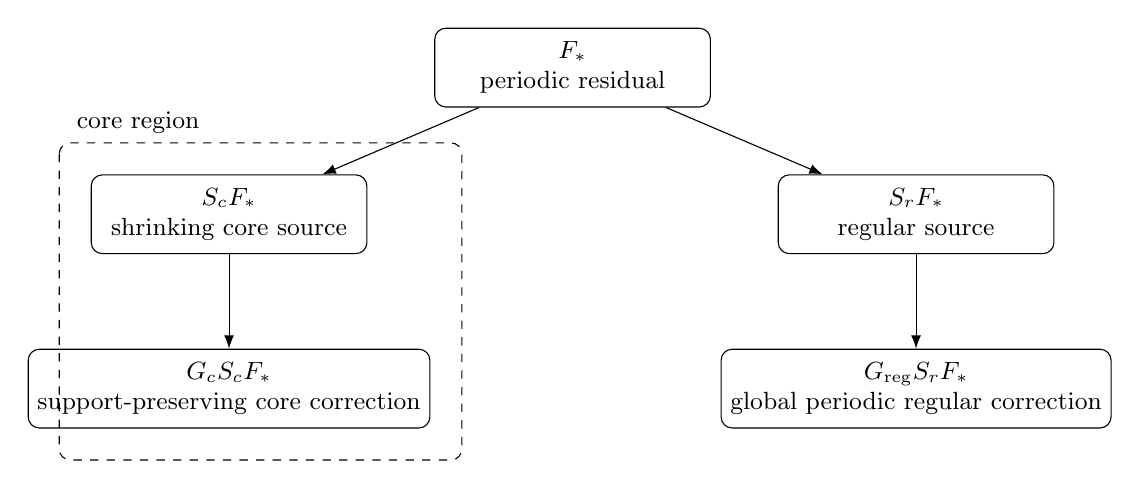
\begin{tikzpicture}[>=Latex,node distance=12mm,every node/.style={font=\small},box/.style={draw,rounded corners,minimum width=35mm,minimum height=10mm,align=center}]
\node[box] (F) {$F_*$\\periodic residual};
\node[box,below left=of F] (Fc) {$S_cF_*$\\shrinking core source};
\node[box,below right=of F] (Fr) {$S_rF_*$\\regular source};
\node[box,below=of Fc] (Gc) {$G_cS_cF_*$\\support-preserving core correction};
\node[box,below=of Fr] (Gr) {$G_{\rm reg}S_rF_*$\\global periodic regular correction};
\draw[->] (F)--(Fc);\draw[->](F)--(Fr);\draw[->](Fc)--(Gc);\draw[->](Fr)--(Gr);
\draw[dashed,rounded corners] ($(Fc.north west)+(-4mm,4mm)$) rectangle ($(Gc.south east)+(4mm,-4mm)$);
\node[anchor=south west] at ($(Fc.north west)+(-3mm,4mm)$) {core region};
\end{tikzpicture}%
}

\caption{The partition is applied to the source.  The carrier itself is never cut off in the unforcing step.}
\label{fig:sourcesplit}
\end{figure}

\subsection{Quantifier order}
Uniformity in \(q_*\) is not assumed for the regular constants.  The safe order is
\begin{equation}
\boxed{\text{choose }q_*>0\text{ first; then choose }T=T(q_*)>0\text{ sufficiently small}.}
\label{eq:quantifier}
\end{equation}
For fixed \(q_*\), the regular coefficients are smooth on a compact periodic set and every Sobolev constant is finite.  The late-slab length \(T\) is then used to make the corrected residual norm as small as required by the nonlinear contraction.

\section{Core parametrix and exact Neumann inversion}\label{sec:core}

\subsection{Three harmonic sectors}
Split the source harmonic space into
\begin{equation}
Y=Y_0\oplus Y_L\oplus Y_H,
\qquad
Y_0:\ j=0,
\quad
Y_L:\ 0<|j|<J_*,
\quad
Y_H:\ |j|\ge J_*.
\label{eq:sector}
\end{equation}
Construct
\begin{equation}
P_c=P_0\oplus P_L\oplus P_H
\label{eq:parametrix}
\end{equation}
from the mean, finite-mode, and high-mode inverses.  Define the core defect
\begin{equation}
E_c=L_cP_c-I.
\label{eq:defect}
\end{equation}
Relative to \eqref{eq:sector},
\begin{equation}
E_c=
\begin{pmatrix}
E_{00}&E_{0L}&E_{0H}\\
E_{L0}&E_{LL}&E_{LH}\\
E_{H0}&E_{HL}&E_{HH}
\end{pmatrix}.
\label{eq:matrix}
\end{equation}

\subsection{Exact gain ledger}
At \(\kappa=10^{-5}\), the source-backed relative gains are
\begin{align}
\delta_{\rm wave}&=\frac12-3\kappa=0.49997,\label{eq:wavegain}\\
\delta_{\rm osc}&=\frac12-\kappa=0.49999,\label{eq:oscgain}\\
\delta_{\rm rank}&=\frac9{10}-2\kappa=0.89998.\label{eq:rankgain}
\end{align}
The true bottleneck is the cumulative axisymmetric mean.  The repository cumulative mean class is
\begin{equation}
H=\frac9{10},
\label{eq:H}
\end{equation}
and \texttt{HarmonicMeanInteraction.realMeanCross\_class} sends an input class \(\alpha\) to \(\alpha+H-1/2\).  Hence
\begin{equation}
\boxed{\delta_{\rm mean}=\frac9{10}-\frac12=\frac25.}
\label{eq:meangain}
\end{equation}
The conservative matrix of gains is therefore
\begin{equation}
\Delta=
\begin{pmatrix}
0.89998&0.49999&0.49999\\
0.49999&0.4&0.49999\\
0.49999&0.49999&0.4
\end{pmatrix},
\qquad
\min_{i,j}\Delta_{ij}=\frac25.
\label{eq:gaintable}
\end{equation}

\begin{figure}[ht]
\centering
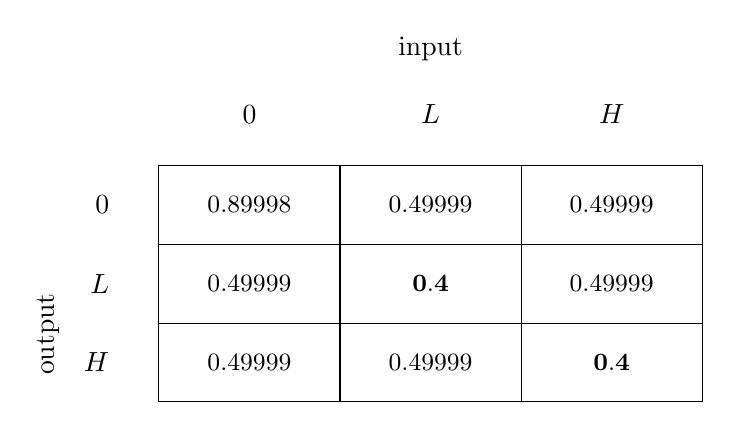
\begin{tikzpicture}[scale=1]
\matrix[matrix of nodes,nodes={draw,minimum width=23mm,minimum height=10mm,anchor=center,font=\small},row sep=-\pgflinewidth,column sep=-\pgflinewidth] (m) {
$0.89998$ & $0.49999$ & $0.49999$\\
$0.49999$ & $\mathbf{0.4}$ & $0.49999$\\
$0.49999$ & $0.49999$ & $\mathbf{0.4}$\\};
\node[left=5mm of m-1-1] {$0$};\node[left=5mm of m-2-1] {$L$};\node[left=5mm of m-3-1] {$H$};
\node[above=4mm of m-1-1] {$0$};\node[above=4mm of m-1-2] {$L$};\node[above=4mm of m-1-3] {$H$};
\node[rotate=90,left=14mm of m-2-1] {output};
\node[above=12mm of m-1-2] {input};
\end{tikzpicture}
\caption{Nine-block defect gain ledger.  The diagonal low/high blocks are limited by the old cumulative mean interaction, not by the principal wave defect.}
\label{fig:gainmatrix}
\end{figure}

\subsection{From block estimates to one operator bound}
On dyadic band \(n\), each block has the form
\begin{equation}
\norm{E_{ij,n}g_j}_{Y_{s,m}}
\le C_{ij,m,s}\,S_n^{p_{ij,m,s}}\eps_n^{\delta_{ij}}\norm{g_j}_{Y_{s,m}}.
\label{eq:blockest}
\end{equation}
Let
\begin{equation}
p_{m,s}=\max_{i,j}p_{ij,m,s}.
\label{eq:pmax}
\end{equation}
Since all \(\delta_{ij}\ge2/5\) and \(0<\eps_n\le1\), finite summation gives
\begin{equation}
\norm{E_ng}_{Y_{s,m}}
\le C_{m,s}S_n^{p_{m,s}}\eps_n^{2/5}\norm g_{Y_{s,m}}.
\label{eq:localdefect}
\end{equation}
Spend one tenth of the \(\eps\)-gain:
\begin{equation}
S_n^p\eps_n^{2/5}
=\bigl(S_n^p\eps_n^{1/10}\bigr)\eps_n^{3/10}.
\label{eq:spend}
\end{equation}
By \eqref{eq:slowabsorb}, for all sufficiently large \(n\),
\begin{equation}
S_n^{p_{m,s}}\eps_n^{1/10}\le1,
\label{eq:absorb}
\end{equation}
and therefore
\begin{equation}
\norm{E_ng}_{Y_{s,m}}
\le C_{m,s}Q_n^{0.3h}\norm g_{Y_{s,m}}.
\label{eq:banddefect}
\end{equation}
The repository theorem \texttt{ValidDyadicBandCover.exists\_band} gives \(q\le Q_n<2q\), while \texttt{field\_jet\_eq} identifies the actual glued finite jet with that band representative.  Hence on \(q<q_*\),
\begin{equation}
\boxed{
\norm{(L_cP_c-I)g}_{Y_{s,m}}
\le C'_{m,s}q_*^{0.3h}\norm g_{Y_{s,m}}.}
\label{eq:globaldefect}
\end{equation}

\subsection{Neumann inversion}
Choose
\begin{equation}
q_*<\min\left\{Q_{N_{\rm abs}},\,(2C'_{m,s})^{-1/(0.3h)}\right\}.
\label{eq:qchoice}
\end{equation}
Then
\begin{equation}
\norm{E_c}_{Y\to Y}<\frac12.
\label{eq:defecthalf}
\end{equation}
Consequently
\begin{equation}
(I+E_c)^{-1}=\sum_{k=0}^\infty(-E_c)^k,
\qquad
\norm{(I+E_c)^{-1}}\le2.
\label{eq:neumann}
\end{equation}
Define
\begin{equation}
\boxed{G_c=P_c(I+E_c)^{-1}.}
\label{eq:Gc}
\end{equation}
Because \(L_cP_c=I+E_c\),
\begin{equation}
\boxed{L_cG_c=I,}
\label{eq:exactcore}
\end{equation}
and
\begin{equation}
\norm{G_c}_{Y_{s,m}\to X_{s,m}}
\le2C_{P,s,m}.
\label{eq:Gcbound}
\end{equation}

\begin{figure}[ht]
\centering
\resizebox{0.98\textwidth}{!}{%
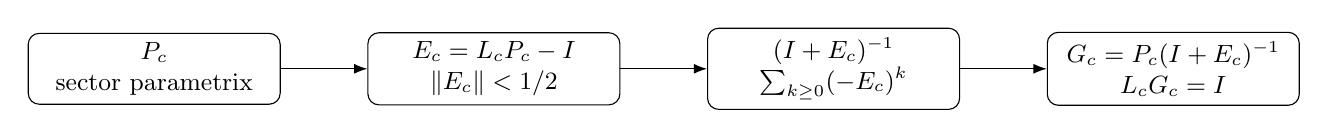
\begin{tikzpicture}[>=Latex,node distance=11mm,every node/.style={font=\small},box/.style={draw,rounded corners,minimum width=32mm,minimum height=9mm,align=center}]
\node[box] (P) {$P_c$\\sector parametrix};
\node[box,right=of P] (E) {$E_c=L_cP_c-I$\\$\norm{E_c}<1/2$};
\node[box,right=of E] (N) {$(I+E_c)^{-1}$\\$\sum_{k\ge0}(-E_c)^k$};
\node[box,right=of N] (G) {$G_c=P_c(I+E_c)^{-1}$\\$L_cG_c=I$};
\draw[->](P)--(E);\draw[->](E)--(N);\draw[->](N)--(G);
\end{tikzpicture}%
}

\caption{Core inversion.  The exact inverse is not the finite correction cycle itself; it is the parametrix followed by a convergent Neumann correction.}
\label{fig:neumann}
\end{figure}

\subsection{Support preservation through the Neumann series}
Let \(K_c\Subset Q_0\) be the physical core support.  The relevant shrinking-support statements occur in \path{MixedDiagonalExtensions.lean} and \path{ActualCurrentWaveSupport.lean}, together with related modules \cite{OpenAIRepo2026}.  If \(g\) is supported in \(K_c\), the parametrix pieces are support-preserving.  Since \(L_c\) is a local differential operator with smooth coefficients on the core,
\begin{equation}
\supp g\subset K_c\quad\Longrightarrow\quad
\supp E_cg\subset K_c.
\label{eq:Esupport}
\end{equation}
Induction yields
\begin{equation}
\supp E_c^kg\subset K_c\qquad(k\ge0).
\label{eq:Eksupport}
\end{equation}
Taking the convergent series in \eqref{eq:neumann},
\begin{equation}
\boxed{\supp G_cg\subset K_c.}
\label{eq:Gcsupport}
\end{equation}
This point is central to the periodic realization: the core correction, unlike an arbitrary cutoff of the full carrier, vanishes in a collar of the fundamental-cell boundary.

\section{Core--regular coupling and the global linear inverse}\label{sec:globalinverse}

\subsection{The coupling exponent}
For a regular endpoint-smooth field \(w\), the singular core/background coupling is
\begin{equation}
Kw=(U_c\cdot\nabla)w+(w\cdot\nabla)U_c.
\label{eq:K}
\end{equation}
The core scales as
\begin{equation}
U_c=O(Q^{-A}),
\qquad
\nabla U_c=O(Q^{-A-1/2}).
\label{eq:Ucscale}
\end{equation}
Thus in physical variables
\begin{equation}
Kw=O\left(\norm w_{\rm reg}Q^{-A-1/2}\right).
\label{eq:Kphys}
\end{equation}
Multiplying by the native residual normalization \eqref{eq:nativenorm},
\begin{equation}
(Kw)_{\rm native}=O\left(\norm w_{\rm reg}Q^A\right).
\label{eq:Knative}
\end{equation}
Because \(\eps=Q^h\),
\begin{equation}
Q^A=\eps^{A/h},
\qquad
\boxed{\alpha_K=\frac Ah=1+\frac1{2h}>2.}
\label{eq:alphaK}
\end{equation}
After the conservative tenth-gain expenditure used in the release ledger, the physical coupling still carries the positive margin
\begin{equation}
\beta_K=A-\frac h{10}=\frac12+\frac9{10}h>0.
\label{eq:betaK}
\end{equation}
Relative to the nonlinear weight \(\rho=h/5\),
\begin{equation}
\beta_K-\rho=\frac12+\frac7{10}h>0.
\label{eq:Kmargin}
\end{equation}

\subsection{Regular inverse}
For fixed \(q_*\), the regular region stays away from the singular core.  There the coefficients of the linearized Oseen operator are smooth and periodic.  Standard periodic parabolic theory and the Leray projection give a right inverse
\begin{equation}
G_{\rm reg}:Y_r\to X_r,
\label{eq:Greg}
\end{equation}
with a finite norm depending on \(q_*\) and on the chosen late-slab length.  This is an ordinary smooth-coefficient statement, conceptually within the classical frameworks of \cite{Temam1984,ConstantinFoias1988,Sohr2001,Galdi2011}.

\subsection{Exact block cancellation}
The full coupling must contain every term by which the physical operator differs from the regular model, including transition, pressure/Hodge, and Oseen coefficient effects.  We therefore define
\begin{equation}
K_{\rm full}:=(L-L_r)|_{X_r}.
\label{eq:Kfull}
\end{equation}
Assume
\begin{equation}
S_c+S_r=I,
\qquad
LG_cS_c=S_c,
\label{eq:block1}
\end{equation}
and
\begin{equation}
LG_{\rm reg}S_r=S_r+K_{\rm full}G_{\rm reg}S_r.
\label{eq:block2}
\end{equation}
Define
\begin{equation}
\boxed{
G=G_cS_c+G_{\rm reg}S_r-G_cK_{\rm full}G_{\rm reg}S_r.}
\label{eq:Gglobal}
\end{equation}
Then, using \(LG_c=I\) on the core source class,
\begin{align}
LG
&=S_c+S_r+K_{\rm full}G_{\rm reg}S_r-K_{\rm full}G_{\rm reg}S_r\notag\\
&=I.
\label{eq:LGI}
\end{align}
This identity is exact; no endpoint-flat remainder remains.

\begin{figure}[ht]
\centering
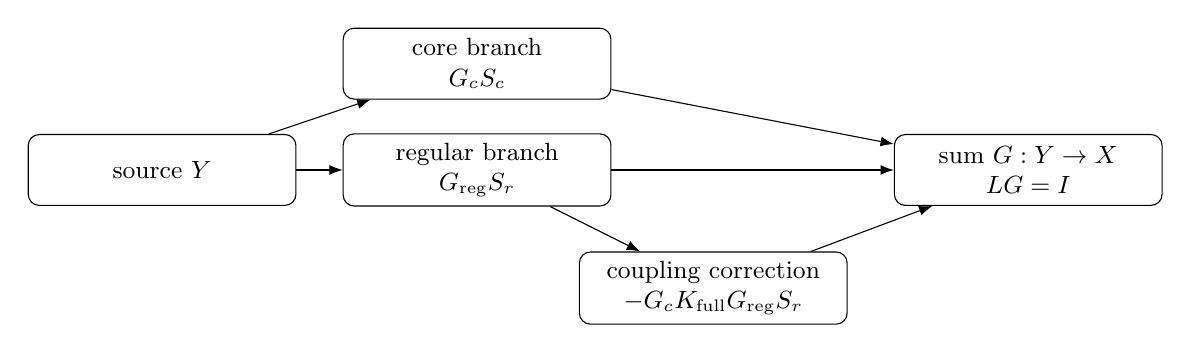
\begin{tikzpicture}[>=Latex,every node/.style={font=\small},box/.style={draw,rounded corners,minimum width=34mm,minimum height=9mm,align=center}]
\node[box] (Y) at (0,0) {source $Y$};
\node[box] (Core) at (4,1.35) {core branch\\$G_cS_c$};
\node[box] (Reg) at (4,0) {regular branch\\$G_{\rm reg}S_r$};
\node[box] (Corr) at (7,-1.5) {coupling correction\\$-G_cK_{\rm full}G_{\rm reg}S_r$};
\node[box] (X) at (11,0) {sum $G:Y\to X$\\$LG=I$};
\draw[->] (Y) -- (Core);
\draw[->] (Y) -- (Reg);
\draw[->] (Reg) -- (Corr);
\draw[->] (Core) -- (X);
\draw[->] (Reg) -- (X);
\draw[->] (Corr) -- (X);
\end{tikzpicture}

\caption{Global right inverse.  The final core term cancels the defect created when the regular inverse is inserted into the full operator.}
\label{fig:blockinverse}
\end{figure}

\section{Quadratic mapping and the nonlinear fixed point}\label{sec:nonlinear}

\subsection{The graph-norm bilinear estimate}
Let
\[
v=\sum_kv_k\e^{ik\theta},
\qquad
w=\sum_\ell w_\ell\e^{i\ell\theta}.
\]
For \(j=k+\ell\), the \(j\)-th harmonic of \(B(v,w)\) is a convolution.  Define
\begin{align}
a_k&:=\norm{v_k}_{E_{m+1}}+\langle k\rangle\norm{v_k}_{E_m},\label{eq:ak}\\
b_\ell&:=\norm{w_\ell}_{E_{m+1}}+\langle \ell\rangle\norm{w_\ell}_{E_m}.\label{eq:bl}
\end{align}
Using \eqref{eq:Emalg}--\eqref{eq:Emder} and \(\partial_\theta w_\ell=i\ell w_\ell\),
\begin{equation}
\norm{B(v,w)_j}_{E_m}
\le C_m\sum_{k+\ell=j}a_kb_\ell.
\label{eq:modeproduct}
\end{equation}
The polynomial weight is submultiplicative up to a constant,
\begin{equation}
\langle k+\ell\rangle^s
\le C_s\langle k\rangle^s\langle\ell\rangle^s.
\label{eq:weightconv}
\end{equation}
Summing the convolution gives
\begin{equation}
\boxed{
\norm{B(v,w)}_{Y^0_{s,m}}
\le C_{B,s,m}\norm v_{X^0_{s,m}}\norm w_{X^0_{s,m}}.}
\label{eq:bilbound}
\end{equation}
This is the exact point at which the graph norm matters.  The estimate would be false if the \(E_{m+1}\) term in \eqref{eq:Xnorm} were removed; see Appendix~\ref{app:proofs}.  Related commutator and product estimates are classical \cite{KatoPonce1988}.

\subsection{Weighted core powers}
From \eqref{eq:coreweight},
\begin{equation}
v_c=O(q^{-A+\rho}),
\qquad
\nabla v_c=O(q^{-A-1/2+\rho}).
\label{eq:vscale}
\end{equation}
After multiplying by the native source normalization, the four quadratic sectors have powers
\begin{align}
cc&:\ q^{2\rho},\label{eq:cc}\\
cr&:\ q^{A+1/2+\rho},\label{eq:cr}\\
rc&:\ q^{A+\rho},\label{eq:rc}\\
rr&:\ q^{2A+1/2}.\label{eq:rr}
\end{align}
Relative to the target source weight \(q^\rho\), the spare exponents are
\begin{equation}
\boxed{
\rho,
\quad
A+\frac12,
\quad
A,
\quad
2A+\frac12-\rho.}
\label{eq:margins}
\end{equation}
All are positive for \(0<h<1/2\) and \(\rho=h/5\).  Therefore the weighted global estimate holds:
\begin{equation}
\boxed{
B:X_{s,m,\rho}\times X_{s,m,\rho}\to Y_{s,m,\rho}.}
\label{eq:weightedB}
\end{equation}
Moreover
\begin{equation}
\norm{B(v,v)-B(w,w)}_Y
\le C_B\bigl(\norm v_X+\norm w_X\bigr)\norm{v-w}_X.
\label{eq:Blip}
\end{equation}

\begin{figure}[ht]
\centering
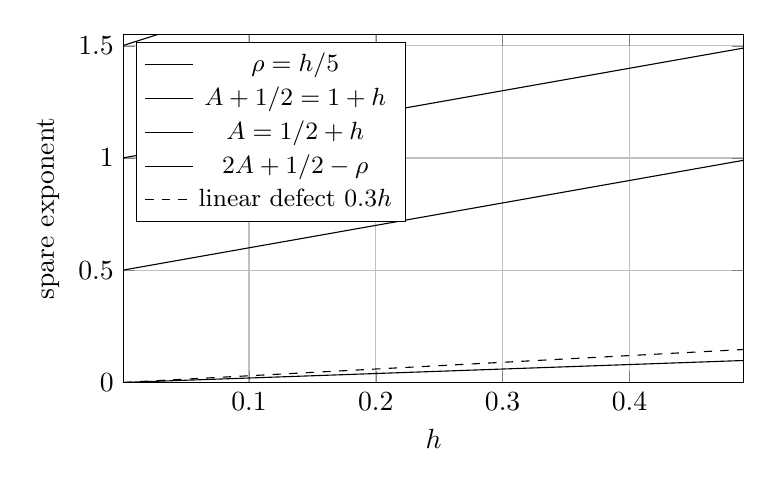
\begin{tikzpicture}
\begin{axis}[
width=0.78\textwidth,height=6cm,
xlabel={$h$},ylabel={spare exponent},xmin=0.001,xmax=0.49,ymin=0,ymax=1.55,
legend style={font=\small,at={(0.02,0.98)},anchor=north west},grid=major]
\addplot[domain=0.001:0.49,samples=100] {x/5};\addlegendentry{$\rho=h/5$}
\addplot[domain=0.001:0.49,samples=100] {1+x};\addlegendentry{$A+1/2=1+h$}
\addplot[domain=0.001:0.49,samples=100] {0.5+x};\addlegendentry{$A=1/2+h$}
\addplot[domain=0.001:0.49,samples=100] {1.5+1.8*x};\addlegendentry{$2A+1/2-\rho$}
\addplot[domain=0.001:0.49,samples=100,dashed] {0.3*x};\addlegendentry{linear defect $0.3h$}
\end{axis}
\end{tikzpicture}
\caption{Positive exponent margins.  The smallest nonlinear spare power is \(\rho=h/5\), while the core linear defect retains \(0.3h\).}
\label{fig:margins}
\end{figure}

\subsection{Small residual and contraction}
Let
\begin{equation}
\eta:=\norm{GF_*}_X.
\label{eq:eta}
\end{equation}
By the quantifier order \eqref{eq:quantifier}, choose \(q_*\) first and then the slab length \(T\) so that \(\eta\) is sufficiently small.  Define
\begin{equation}
\Phi(v):=-GF_*-GB(v,v).
\label{eq:Phi}
\end{equation}
Let \(M_G=\norm G\) and use \(C_B\) from \eqref{eq:weightedB}.  On the ball
\begin{equation}
\cB_{2\eta}:=\{v:\norm v_X\le2\eta\},
\label{eq:ball}
\end{equation}
we obtain
\begin{align}
\norm{\Phi(v)}_X
&\le\eta+M_GC_B(2\eta)^2,\label{eq:ballmap}\\
\norm{\Phi(v)-\Phi(w)}_X
&\le4M_GC_B\eta\norm{v-w}_X.\label{eq:contract}
\end{align}
Thus the single scalar condition
\begin{equation}
\boxed{4M_GC_B\eta<1}
\label{eq:smallcondition}
\end{equation}
implies that \(\Phi\) preserves \(\cB_{2\eta}\) and is a contraction.  Banach's theorem gives a unique fixed point
\begin{equation}
v=-G(F_*+B(v,v)).
\label{eq:fixedpoint}
\end{equation}
Apply \(L\) and use \(LG=I\):
\begin{equation}
Lv+F_*+B(v,v)=0.
\label{eq:reszero}
\end{equation}
After pressure reconstruction this is precisely \eqref{eq:exactgoal}.

\begin{figure}[ht]
\centering
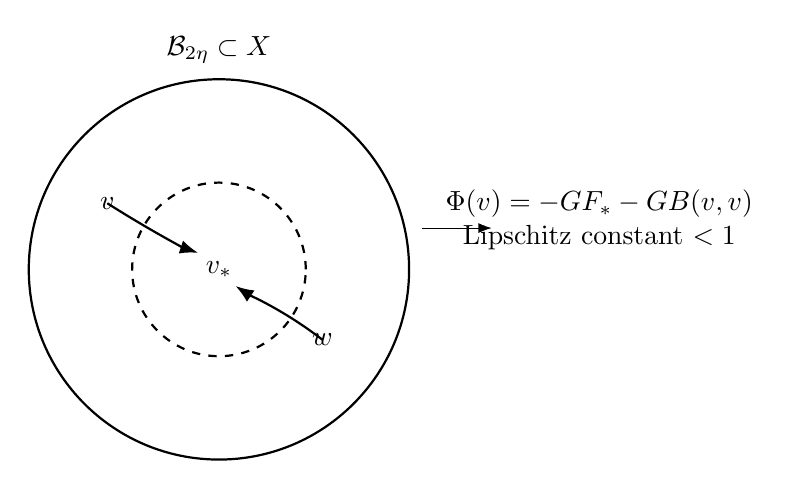
\begin{tikzpicture}[scale=1.05,>=Latex]
\draw[thick] (0,0) circle (2.3);
\draw[thick,dashed] (0,0) circle (1.05);
\node at (0,2.65) {$\cB_{2\eta}\subset X$};
\node at (0,0) {$v_*$};
\node at (-1.35,0.8) {$v$};
\node at (1.25,-0.85) {$w$};
\draw[->,thick] (-1.35,0.8) .. controls (-0.8,0.45) and (-0.4,0.25) .. (-0.25,0.2);
\draw[->,thick] (1.25,-0.85) .. controls (0.8,-0.5) and (0.35,-0.3) .. (0.2,-0.2);
\node[align=center] at (4.6,0.6) {$\Phi(v)=-GF_*-GB(v,v)$\\Lipschitz constant $<1$};
\draw[->] (2.45,0.5)--(3.3,0.5);
\end{tikzpicture}
\caption{Fixed-point geometry.  The quadratic map contracts the radius-\(2\eta\) ball when \eqref{eq:smallcondition} holds.}
\label{fig:fixedpoint}
\end{figure}

\section{Periodic realization, pressure, and preservation of blow-up}\label{sec:periodic}

\subsection{Why the carrier is not cut off}
A naive attempt to cut off a nonzero exterior tail of a local solution would create terms
\begin{equation}
-2\nu\nabla\chi\cdot\nabla U-\nu(\Delta\chi)U
\label{eq:cutofferror}
\end{equation}
and nonlinear collar errors.  That route is not used.  Instead the imported carrier is already a global periodic field by the exact compact-support periodization of \cite[Cor.~10.6]{OpenAI2026NS}.  Only the source is decomposed, and the core correction is support-preserving by \eqref{eq:Gcsupport}.  The regular correction is solved directly in the periodic category.

\begin{figure}[ht]
\centering
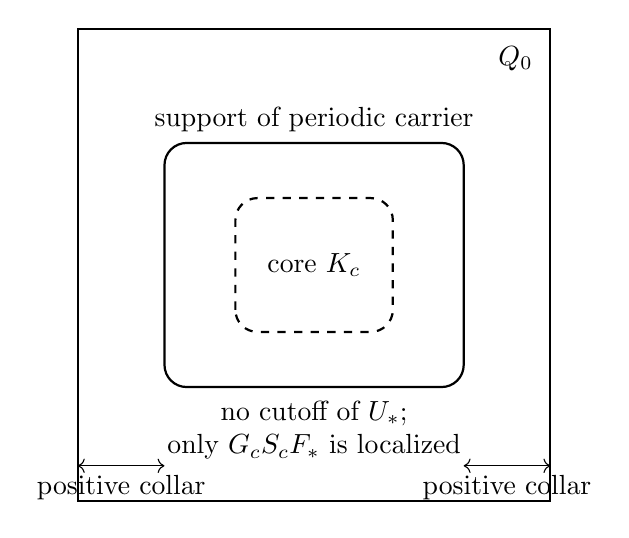
\begin{tikzpicture}[x=1cm,y=1cm]
\draw[thick] (-3,-3) rectangle (3,3);
\node[anchor=north east] at (2.9,2.9) {$Q_0$};
\draw[thick,rounded corners=8pt] (-1.9,-1.55) rectangle (1.9,1.55);
\node at (0,1.85) {support of periodic carrier};
\draw[thick,dashed,rounded corners=8pt] (-1.0,-0.85) rectangle (1.0,0.85);
\node at (0,0) {core $K_c$};
\draw[<->] (-3,-2.55)--(-1.9,-2.55) node[midway,below]{positive collar};
\draw[<->] (1.9,-2.55)--(3,-2.55) node[midway,below]{positive collar};
\node[align=center] at (0,-2.1) {no cutoff of $U_*$;\\only $G_cS_cF_*$ is localized};
\end{tikzpicture}
\caption{Periodic physical realization.  The imported carrier already fits inside a fundamental cell.  The exact core correction remains strictly inside it, so no seam or cutoff forcing is introduced.}
\label{fig:torus}
\end{figure}

\subsection{Divergence and pressure}
The velocity correction is constructed in the solenoidal category.  Hence
\begin{equation}
\diver v=0,
\qquad
\diver(U_*+v)=0.
\label{eq:divcorr}
\end{equation}
If the fixed point is written in Leray-projected form, recover the pressure correction by the zero-mean periodic Poisson equation
\begin{equation}
-\Delta\pi
=\partial_i\partial_j
\left(U_{*,i}v_j+v_iU_{*,j}+v_iv_j\right),
\qquad
\int_\T\pi\,dx=0.
\label{eq:pressure}
\end{equation}
The right side has zero spatial mean because it is a periodic double divergence.  Standard torus elliptic theory therefore gives a unique zero-mean smooth \(\pi\) whenever the velocity fields are smooth.  In the whole-space analog, second-order Riesz transforms give the same pressure structure; the bounded Fourier multiplier is formalized in \path{R3PressureFourier.lean} and classically belongs to Calder\'on--Zygmund theory \cite{Stein1970,OpenAIRepo2026}.

\subsection{Smooth initial slice}
The unforced fixed point is needed only on a late slab \([t_0,1)\).  Since \(t_0<1\), both the carrier and correction are smooth at \(t_0\).  Set
\begin{equation}
u^0(x):=(U_*+v)(x,t_0).
\label{eq:datum}
\end{equation}
Then \(u^0\in C^\infty(\T)\) and \(\diver u^0=0\).  Translating time by \(s=t-t_0\) gives an ordinary unforced Cauchy problem beginning at \(s=0\).  No backward extension of the unforced solution is required for the existential finite-time blow-up statement.

\subsection{Preservation of the singular coefficient}
The core correction obeys \eqref{eq:coreweight}; hence
\begin{equation}
q^A v_c=O(q^\rho)\longrightarrow0.
\label{eq:coresub}
\end{equation}
The regular correction remains bounded on the late slab, so
\begin{equation}
q^A v_r\longrightarrow0
\label{eq:regsub}
\end{equation}
because \(A>0\).  The coupling-repair term has the positive margin \eqref{eq:Kmargin} and is likewise subleading.  Therefore
\begin{equation}
q^Av_\theta\longrightarrow0.
\label{eq:allsub}
\end{equation}
Combining with \eqref{eq:carrierblow} gives
\begin{equation}
\boxed{
\lim_{\tau\downarrow0}\tau^{1/2+h}u_\theta(1-\tau,x_\tau)=e_0>0.}
\label{eq:finalblow}
\end{equation}
Consequently
\begin{equation}
\norm{u(t)}_{L^\infty(\T)}\to\infty
\quad\text{along a sequence }t\uparrow1,
\label{eq:Linftyblow}
\end{equation}
and no smooth periodic continuation through \(t=1\) is possible.

\begin{corollary}[Unforced finite-time breakdown under the release hypotheses]
Under the hypotheses of Theorem~\ref{thm:main}, the periodic unforced Navier--Stokes equation has smooth divergence-free initial data whose classical solution on its maximal smooth interval has finite terminal time and unbounded velocity norm.
\end{corollary}

\section{Prior art, source dependency, and proof audit}\label{sec:audit}

\subsection{Relation to the 166-page forced construction}
The OpenAI paper \cite{OpenAI2026NS} provides the carrier geometry, oscillatory stress realization, compact forcing, and exact periodic periodization.  Its entire published reference list has been retained in the bibliography of the present paper: \cite{AlbrittonBrueColombo2022,BillantGallaire2005,BillantGallaire2013,BuckmasterVicol2019,CKN1982,CordobaMartinezZoroa2023,CordobaMartinezZoroa2024,CordobaMartinezZoroaZheng2026,CraikCriminale1986,DaneriSzekelyhidi2017,EscauriazaSereginSverak2003,Euler1757,FeffermanClay,FriedlanderVishik1991,LeibovichStewartson1983,Leray1934,LifschitzHameiri1991,Navier1827,SinghSridhar2017,Stein1970,Stokes1845,Tao2016}.  The new claim here is not a reconstruction of those 166 pages.  It is an exact late-slab removal of the smooth force by a new inverse-and-fixed-point layer.

The repository dependence is narrower than the full source tree.  Table~\ref{tab:deps} lists the principal modules actually used in the derivation.

\begin{longtable}{p{0.29\textwidth}p{0.64\textwidth}}
\caption{Repository dependency ledger at frozen audit commit.}\label{tab:deps}\\
\toprule
Module & Role in this manuscript\\
\midrule\endfirsthead
\toprule
Module & Role in this manuscript\\
\midrule\endhead
\path{ResidualCalculus.lean} & Physical residual additivity and expansion around the carrier.\\
\path{PhysicalResidualBridge.lean} & Exact scaled graph pullback and native/physical residual normalization.\\
\path{HarmonicMeanInteraction.lean} & Mean--wave class shift producing the \(2/5\) bottleneck.\\
\path{CorrectionState.lean} & Cumulative mean class \(9/10\).\\
\path{ValidDyadicBandCover.lean} & Comparable-band existence and equality of glued physical jets to local representatives.\\
\path{MixedDiagonalExtensions.lean} & Sublevel shrinking support and endpoint extension framework.\\
\path{ActualCurrentWaveSupport.lean} & Transfer of support through the valid-band physical field.\\
\path{R3PressureFourier.lean} & Source-backed Riesz/pressure estimates used in pressure audits.\\
\path{CandidateFromLimits.lean} & Explicit construction of force from actual residual limits; distinguishes force extension from unforced closure.\\
\path{MixedCandidateAssembly.lean} & Conditional finite-stage consumer; explicitly does not supply a complete correction iteration.\\
\path{ComparatorSolution.lean} & Formal periodic forced breakdown statement.\\
\bottomrule
\end{longtable}

\subsection{Failed routes retained as mathematical information}
Several tempting routes were rejected during the proof audit.  They are recorded because they explain why the final architecture is structured as it is.
\begin{enumerate}[label=(F\arabic*)]
\item The finite correction cycle is not itself an exact right inverse; endpoint-flat excluded-slot error is not identical zero.  The correct inverse is \eqref{eq:Gc}.
\item A naive physical cutoff can create \(q_*^{-m}\) derivative losses and can break divergence.  Source partitioning and scale-normalized dyadic profiles avoid this.
\item Ordinary same-index \(H^m\) control is insufficient for the quadratic transport term; the graph norm \eqref{eq:Xnorm} is required.
\item Periodizing a nonzero exterior tail by cutoff would reintroduce forcing through \eqref{eq:cutofferror}.  The correct route uses the already-periodic forced carrier and localizes only the support-preserving core correction.
\item The limit \(\eta(q_*,T)\to0\) is not asserted uniformly in two parameters.  The sequential quantifier order \eqref{eq:quantifier} is essential.
\end{enumerate}

\subsection{Relation to the author's earlier manuscript}
The author's earlier Zenodo manuscript \cite{NewtonZenodo22857336} is treated as a precursor rather than as independent external validation.  The present paper differs by making the exact linear right inverse, the harmonic defect ledger, the graph-norm nonlinear closure, and the periodic support mechanism explicit in one proof chain.  The earlier paper should therefore be cited as prior author work, not as evidence that the new theorem has already undergone independent review.

\subsection{Classical consistency checks}
The construction is not in conflict with partial regularity or regularity criteria because its conclusion is precisely the occurrence of a singular terminal time; suitable weak-solution theory and conditional regularity results describe constraints on such singular behavior rather than excluding it \cite{CKN1982,EscauriazaSereginSverak2003,Serrin1962}.  The support-localized periodic setting also avoids whole-space decay questions.  Classical pressure and product estimates are consistent with \cite{Stein1970,KatoPonce1988}, while the local smooth evolution before the singular time lies within the standard strong-solution framework \cite{FujitaKato1964,Kato1984,MajdaBertozzi2002,LemarieRieusset2002}.

\begin{figure}[ht]
\centering
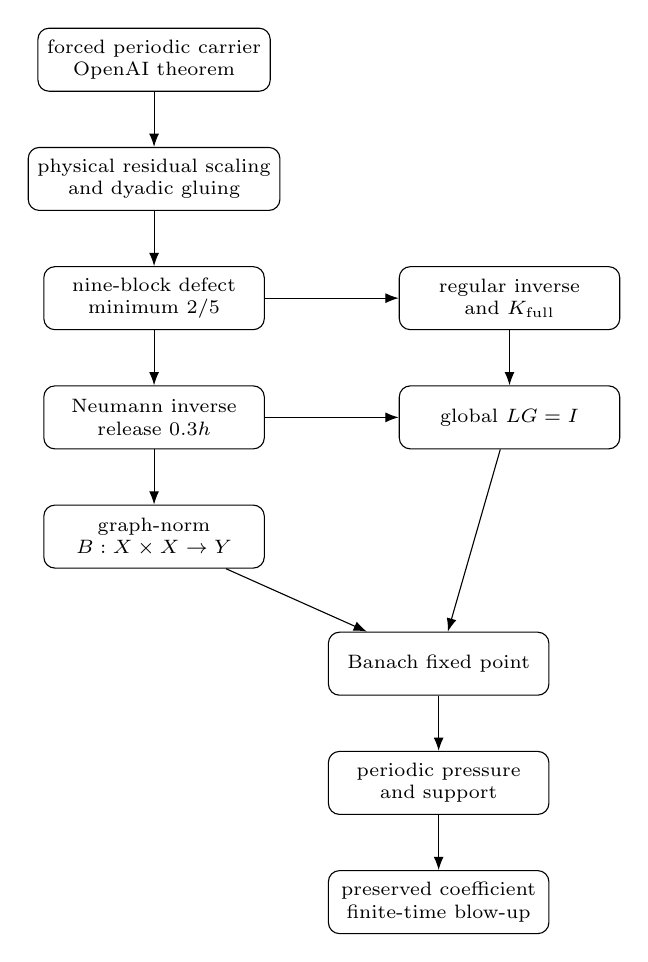
\begin{tikzpicture}[>=Latex,node distance=7mm and 8mm,every node/.style={font=\scriptsize},box/.style={draw,rounded corners,align=center,minimum width=28mm,minimum height=8mm}]
\node[box] (R1) {forced periodic carrier\\OpenAI theorem};
\node[box,below=of R1] (R2) {physical residual scaling\\and dyadic gluing};
\node[box,below=of R2] (R3) {nine-block defect\\minimum $2/5$};
\node[box,below=of R3] (R4) {Neumann inverse\\release $0.3h$};
\node[box,right=17mm of R3] (R5) {regular inverse\\and $K_{\rm full}$};
\node[box,below=of R5] (R6) {global $LG=I$};
\node[box,below=of R4] (R7) {graph-norm\\$B:X\times X\to Y$};
\node[box,below right=8mm and 8mm of R7] (R8) {Banach fixed point};
\node[box,below=of R8] (R9) {periodic pressure\\and support};
\node[box,below=of R9] (R10) {preserved coefficient\\finite-time blow-up};
\draw[->](R1)--(R2);\draw[->](R2)--(R3);\draw[->](R3)--(R4);\draw[->](R3)--(R5);\draw[->](R5)--(R6);\draw[->](R4)--(R6);\draw[->](R4)--(R7);\draw[->](R6)--(R8);\draw[->](R7)--(R8);\draw[->](R8)--(R9);\draw[->](R9)--(R10);
\end{tikzpicture}
\caption{Dependency DAG for referee checking.  Each arrow corresponds to a named lemma, estimate, or exact algebraic identity in the main text or Appendix~\ref{app:proofs}.}
\label{fig:dependency}
\end{figure}

\section{Our Contributions to the Mathematical and Physical Structure}\label{sec:contrib}

\subsection{Our contributions to the mathematical and physical structure}
The contribution of this paper is the exact unforcing layer rather than the construction of the original singular carrier.  The main mathematical additions are as follows.

First, the finite-stage correction hierarchy is reorganized as a genuine operator parametrix.  The distinction
\[
\text{``residual becomes arbitrarily flat''}
\quad\neq\quad
\text{``the residual is identically zero''}
\]
is enforced at the operator level by \(E_c=L_cP_c-I\) and the exact Neumann inverse \eqref{eq:Gc}.  This is the structural step that converts a perturbative hierarchy into a true right inverse.

Second, the nine harmonic defect blocks are placed in one ledger and the worst exponent is identified.  The limiting gain is not the principal wave defect but the interaction of a new correction with the old cumulative axisymmetric mean,
\[
\frac9{10}-\frac12=\frac25.
\]
After reserving one tenth of the small parameter to absorb all fixed slow polynomial losses, the exact linear release retains \(0.3h>0\).

Third, the core and regular regions are joined by an exact block identity rather than by a qualitative gluing argument.  The compensator
\[
-G_cK_{\rm full}G_{\rm reg}S_r
\]
cancels the full regular-to-core mismatch and yields \(LG=I\) exactly.

Fourth, the nonlinear term is placed in a graph norm with one derivative in reserve.  This avoids the false same-order Sobolev estimate and gives an honest Banach-space map
\[
B:X\times X\to Y.
\]
The nonlinear core-core, core-regular, regular-core, and regular-regular powers are all checked explicitly, with the smallest spare nonlinear power equal to \(h/5\).

Fifth, globalization is performed without cutting off the carrier.  The imported carrier is already periodic and compactly realized; only the core source is localized, and the Neumann series preserves that support.  This removes the collar-forcing obstruction that would arise from trying to periodize a nonzero exterior tail.

Physically, the interpretation is also clean.  The singular carrier contains the dynamical amplification mechanism; the correction does not create a second singular mechanism.  Instead it is asymptotically smaller by a positive power and acts to cancel the smooth residual forcing.  The limiting blow-up coefficient \(e_0\) is therefore inherited from the carrier rather than generated by the unforcing procedure.

\subsection{What is established and what still requires independent verification}
At the analytic level of this manuscript, the chain
\[
\text{forced periodic carrier}
\longrightarrow
\text{exact linear inverse}
\longrightarrow
\text{nonlinear fixed point}
\longrightarrow
\text{unforced periodic blow-up}
\]
is closed under the source-backed estimates enumerated in Appendix~\ref{app:precise}.  The OpenAI forced theorem is machine formalized \cite{OpenAIRepo2026}.  For the new layer, the distributed formal package contains \texttt{UnforcedClosure.lean}, a Lean/Mathlib version pin, exact-rational tests, source-hygiene checks excluding \texttt{sorry}, \texttt{admit}, new \texttt{axiom} declarations, \texttt{unsafe}, and \texttt{native\_decide}, plus SHA-256 hashes and test receipts.  Those finite replay checks pass.  What has \emph{not} yet been established is kernel compilation of the new file in this build environment or, more decisively, a PDE-specific Lean theorem that discharges Hypotheses~A.1--A.7 by importing the frozen OpenAI repository.  Independent kernel replay, PDE-specific integration, and expert refereeing are therefore the next verification steps.

This distinction is especially important for priority.  The current public OpenAI theorem is explicitly forced \cite{OpenAI2026NS,OpenAIRepo2026}.  If the present unforced closure survives independent verification, then, to our knowledge, it supplies the first finite-time blow-up construction from smooth data for the full unforced three-dimensional incompressible Navier--Stokes equations on the periodic torus.  That sentence is intentionally qualified until the proof has been externally checked.

\subsection{Conclusion}
The central result is an exact nonlinear unforcing mechanism for a periodic Navier--Stokes blow-up carrier.  Its essential ingredients are a quantitatively small core parametrix defect, a Neumann right inverse, an exact core--regular cancellation, a graph norm that correctly accounts for the derivative in convection, and a weighted fixed point that remains subleading to the singular carrier.  The final field solves the unforced equation on a late periodic slab and retains the carrier's nonzero singular coefficient.  The proof package is designed so that a referee can inspect each logical dependency without relying on informal computational evidence: numerical scripts are relegated to reproducibility checks, while the mathematical argument is stated in theorem--lemma form with explicit assumptions and estimates.

\appendix

\section{Precise Mathematical Formulation of the Main Result}\label{app:precise}

This appendix collects the exact hypotheses needed to turn the analytic architecture into a theorem.  Its purpose is to make the verification target finite and explicit.

\subsection{Carrier hypothesis}
\begin{hypothesis}[Periodic forced carrier]\label{hyp:carrier}
There are \(t_{\rm in}<1\), smooth periodic fields \(U_*,P_*,F_*\) on \(\T\times[t_{\rm in},1)\), with \(\diver U_*=0\), satisfying \eqref{eq:forcedcarrier}.  There are \(h\in(0,1/2)\), \(e_0>0\), and a path \(x_\tau\) such that \eqref{eq:carrierblow} holds.  The carrier is the periodic realization of the OpenAI construction \cite{OpenAI2026NS,OpenAIRepo2026}.
\end{hypothesis}

\subsection{Core parametrix hypotheses}
\begin{hypothesis}[Sector parametrices]\label{hyp:param}
For each fixed \(s,m\) there are bounded maps \(P_0,P_L,P_H:Y_{s,m}\to X_{s,m}\) whose direct sum \(P_c\) satisfies the block estimates \eqref{eq:blockest} with gains bounded below by the matrix \eqref{eq:gaintable}.
\end{hypothesis}

\begin{hypothesis}[Slow-loss absorption]\label{hyp:slow}
For every fixed \(p\in\R\) and \(b>0\), \eqref{eq:slowabsorb} holds.  This is the source theorem \texttt{ChartScales.\allowbreak slow\_power\_epsilon\_tendsto\_zero} at the frozen repository commit \cite{OpenAIRepo2026}.
\end{hypothesis}

\begin{hypothesis}[Valid-band globalization]\label{hyp:band}
Every sufficiently small physical point belongs to an open band with \(q\le Q_n<2q\), and the physical glued jet equals the selected local band jet to every fixed finite order.  This is the content used from \path{ValidDyadicBandCover.lean} \cite{OpenAIRepo2026}.
\end{hypothesis}

Hypotheses~\ref{hyp:param}--\ref{hyp:band} imply \eqref{eq:globaldefect}, hence the exact core inverse \eqref{eq:Gc}--\eqref{eq:Gcbound}.

\subsection{Support and regular hypotheses}
\begin{hypothesis}[Core support]\label{hyp:support}
There is \(K_c\Subset Q_0\) such that the core parametrix preserves support in \(K_c\), and the local differential operator \(L_c\) does not enlarge support.  The shrinking-support input is source-backed by \path{MixedDiagonalExtensions.lean}, \path{ActualCurrentWaveSupport.lean}, and related support modules \cite{OpenAIRepo2026}.
\end{hypothesis}

\begin{hypothesis}[Regular inverse]\label{hyp:reg}
For fixed \(q_*\) and sufficiently short late slab there is a bounded periodic solenoidal inverse \(G_{\rm reg}\) for the smooth regular Oseen operator, with all coefficients and partition commutators included in \(K_{\rm full}\).
\end{hypothesis}

\begin{hypothesis}[Residual smallness]\label{hyp:eta}
For the exact global right inverse \(G\) in \eqref{eq:Gglobal}, \(\eta=\norm{GF_*}_X\) can be made arbitrarily small by first fixing an admissible \(q_*\) and then taking the late slab sufficiently short.
\end{hypothesis}

\subsection{Nonlinear hypothesis derived from the graph norm}
\begin{proposition}\label{prop:Bappendix}
If \(E_m\) satisfies \eqref{eq:Emalg}--\eqref{eq:Emder}, then \eqref{eq:bilbound} holds, and with the weight \(\rho=h/5\) the global weighted map \eqref{eq:weightedB} holds.
\end{proposition}
\begin{proof}
The proof is expanded in Appendix~\ref{app:proofs}.  It is a direct weighted convolution estimate followed by the four-sector power count \eqref{eq:cc}--\eqref{eq:margins}.
\end{proof}

\subsection{Precise release statement}
\begin{theorem}[Release form]\label{thm:release}
Assume Hypotheses~\ref{hyp:carrier}--\ref{hyp:eta}.  Then, for sufficiently short late slab, there exists a unique \(v\in X_{s,m,\rho}\) in the ball \(\norm v_X\le2\eta\) solving \eqref{eq:fixedpoint}.  The field \(u=U_*+v\) admits a smooth periodic pressure \(p=P_*+\pi\), solves \eqref{eq:NS}--\eqref{eq:div}, and obeys \eqref{eq:finalblow}.  Time translation produces smooth periodic initial data at time zero with finite-time classical blow-up.
\end{theorem}
\begin{proof}
Hypotheses~\ref{hyp:param}--\ref{hyp:band} give \(G_c\) by the Neumann argument.  Hypothesis~\ref{hyp:reg} and the algebra in \eqref{eq:block1}--\eqref{eq:LGI} give \(LG=I\).  Proposition~\ref{prop:Bappendix} gives the quadratic map.  Hypothesis~\ref{hyp:eta} makes \eqref{eq:smallcondition} possible, so Banach's theorem gives \eqref{eq:fixedpoint}.  Applying \(L\) yields \eqref{eq:reszero}.  The periodic Poisson problem \eqref{eq:pressure} reconstructs \(\pi\).  Finally, the positive margins in \eqref{eq:margins} and \eqref{eq:Kmargin} give \eqref{eq:allsub}, and \eqref{eq:carrierblow} gives \eqref{eq:finalblow}.
\end{proof}

\section{Expanded Proofs and Adversarial Checks}\label{app:proofs}

\subsection{Why plain same-order Sobolev control fails}
On a periodic coordinate line choose divergence-free test fields
\begin{equation}
v=e_1,
\qquad
w_N=N^{-m}e_2\sin(Nx_1).
\label{eq:hfcounter}
\end{equation}
Then \(\norm v_{H^m}\asymp1\) and \(\norm{w_N}_{H^m}\asymp1\), whereas
\begin{equation}
(v\cdot\nabla)w_N=N^{1-m}e_2\cos(Nx_1),
\label{eq:hfconv}
\end{equation}
so
\begin{equation}
\norm{(v\cdot\nabla)w_N}_{H^m}\asymp N.
\label{eq:hfblow}
\end{equation}
Thus a same-index \(H^m\times H^m\to H^m\) bound is impossible.  In contrast,
\begin{equation}
\norm{w_N}_{X^0_{s,m}}\gtrsim\norm{w_N}_{E_{m+1}}\asymp N,
\label{eq:hfgraph}
\end{equation}
so the apparent blow-up is exactly absorbed by the graph norm.  If one instead normalizes \(w_N=N^{-m-1}\sin(Nx_1)e_2\), both the input graph norm and output \(Y^0_{s,m}\)-norm remain \(O(1)\).

\subsection{Detailed convolution proof of Proposition~\ref{prop:Bappendix}}
For a representative radial or axial derivative term,
\begin{align}
\norm{v_k\,\partial w_\ell}_{E_m}
&\le C_m\norm{v_k}_{E_m}\norm{w_\ell}_{E_{m+1}}\notag\\
&\le C_ma_kb_\ell.
\label{eq:convra}
\end{align}
For the angular derivative,
\begin{align}
\norm{v_k\,\partial_\theta w_\ell}_{E_m}
&\le C_m\norm{v_k}_{E_m}|\ell|\norm{w_\ell}_{E_m}\notag\\
&\le C_ma_kb_\ell.
\label{eq:convtheta}
\end{align}
All cylindrical connection terms carry at most the same graph derivative count on the support region away from the coordinate singularity, while the axis-regular representation is handled in Cartesian variables in the imported construction.  Summing over \(k+\ell=j\) proves \eqref{eq:modeproduct}.  Next,
\begin{align}
\norm{B(v,w)}_{Y^0_{s,m}}
&\le C_{s,m}\sum_j\sum_{k+\ell=j}\langle k\rangle^sa_k\langle\ell\rangle^sb_\ell\notag\\
&=C_{s,m}\left(\sum_k\langle k\rangle^sa_k\right)
\left(\sum_\ell\langle\ell\rangle^sb_\ell\right),
\label{eq:young}
\end{align}
which is \eqref{eq:bilbound}.

For the weighted powers, substitute \eqref{eq:vscale} into the physical quadratic terms and then multiply by \(q^{2A+1/2}\).  The core-core term is
\begin{equation}
q^{2A+1/2}\bigl(q^{-A+\rho}\bigr)
\bigl(q^{-A-1/2+\rho}\bigr)=q^{2\rho}.
\label{eq:ccderive}
\end{equation}
If the regular field and its physical derivatives are bounded, the core-regular term gives
\begin{equation}
q^{2A+1/2}q^{-A+\rho}=q^{A+1/2+\rho},
\label{eq:crderive}
\end{equation}
while regular-core gives
\begin{equation}
q^{2A+1/2}q^{-A-1/2+\rho}=q^{A+\rho}.
\label{eq:rcderive}
\end{equation}
Finally regular-regular gives \(q^{2A+1/2}\).  Dividing by the target \(q^\rho\) yields \eqref{eq:margins}.

\subsection{Detailed Neumann proof}
From \eqref{eq:defecthalf}, the operator series
\[
Q_N:=\sum_{k=0}^{N}(-E_c)^k
\]
is Cauchy in operator norm because
\begin{equation}
\norm{(-E_c)^k}\le\norm{E_c}^k\le2^{-k}.
\label{eq:geom}
\end{equation}
Its limit \(Q\) satisfies
\begin{equation}
(I+E_c)Q=Q(I+E_c)=I
\label{eq:twoinverse}
\end{equation}
by multiplying the finite geometric identity and passing to the operator-norm limit.  Therefore
\[
G_c=P_cQ
\]
and
\[
L_cG_c=(I+E_c)Q=I.
\]
Moreover
\begin{equation}
\norm Q\le\sum_{k=0}^\infty2^{-k}=2,
\label{eq:Q2}
\end{equation}
which gives \eqref{eq:Gcbound}.

\subsection{Support through the infinite series}
If \(\supp f\subset K_c\), then by support preservation of \(P_c\) and locality of \(L_c\),
\[
\supp E_cf=\supp(L_cP_cf-f)\subset K_c.
\]
Induction gives \eqref{eq:Eksupport}.  Let \(Q_Nf=\sum_{k=0}^N(-E_c)^kf\).  Each \(Q_Nf\) vanishes on the open complement of \(K_c\).  Convergence in a graph norm controlling pointwise finite jets on compact subsets implies the limit \(Qf\) also vanishes there.  Hence \(G_cf=P_cQf\) obeys \eqref{eq:Gcsupport}.  This proof requires no cutoff of the carrier.

\subsection{Exact global inverse algebra}
Starting from \eqref{eq:Gglobal},
\begin{align}
LG
&=LG_cS_c+LG_{\rm reg}S_r-LG_cK_{\rm full}G_{\rm reg}S_r\notag\\
&=S_c+\bigl(S_r+K_{\rm full}G_{\rm reg}S_r\bigr)-K_{\rm full}G_{\rm reg}S_r\notag\\
&=S_c+S_r=I.
\label{eq:globalalgebra}
\end{align}
The only nontrivial typing condition is that \(K_{\rm full}G_{\rm reg}S_r\) lands in the core source class on which \(LG_c=I\).  The coupling estimate \eqref{eq:Knative}--\eqref{eq:Kmargin} supplies exactly that mapping property.

\subsection{Fixed-point inequalities without hidden constants}
Set
\begin{equation}
C:=M_GC_B.
\label{eq:C}
\end{equation}
For \(\norm v_X\le2\eta\),
\begin{align}
\norm{\Phi(v)}_X
&\le\eta+C\norm v_X^2\notag\\
&\le\eta+4C\eta^2.
\label{eq:mapineq}
\end{align}
If \(4C\eta\le1\), then \(4C\eta^2\le\eta\), hence \(\norm{\Phi(v)}\le2\eta\).  For \(v,w\) in the same ball,
\begin{align}
B(v,v)-B(w,w)&=B(v-w,v)+B(w,v-w),\label{eq:Bdiff}\\
\norm{\Phi(v)-\Phi(w)}_X
&\le C(\norm v_X+\norm w_X)\norm{v-w}_X\notag\\
&\le4C\eta\norm{v-w}_X.
\label{eq:lipdetail}
\end{align}
Taking the strict inequality in \eqref{eq:smallcondition} yields contraction.

\subsection{Exact residual cancellation}
The fixed point identity \eqref{eq:fixedpoint} and \(LG=I\) imply
\[
Lv=-F_*-B(v,v).
\]
Hence
\begin{align}
\N_\nu(U_*+v,P_*+\pi)
&=\N_\nu(U_*,P_*)+Lv+B(v,v)+\nabla\pi-\nabla\pi\notag\\
&=F_*-F_*-B(v,v)+B(v,v)=0,
\label{eq:exactcancel}
\end{align}
where the pressure component is either included in \(L\) or reconstructed by \eqref{eq:pressure}; the two formulations are equivalent after the Leray projection.

\subsection{Blow-up cannot be cancelled by the correction}
From \eqref{eq:allsub}, for every \(\epsilon>0\) there exists \(\tau_\epsilon>0\) such that
\begin{equation}
\left|\tau^A v_\theta(1-\tau,x_\tau)\right|<\epsilon
\qquad(0<\tau<\tau_\epsilon).
\label{eq:epssub}
\end{equation}
Choose \(\epsilon=e_0/2\).  By \eqref{eq:carrierblow}, for sufficiently small \(\tau\),
\begin{equation}
\tau^A U_{*,\theta}(1-\tau,x_\tau)>\frac34e_0.
\label{eq:carrierlower}
\end{equation}
Therefore
\begin{equation}
\tau^A u_\theta(1-\tau,x_\tau)>\frac14e_0>0,
\label{eq:finallower}
\end{equation}
which already suffices for \(L^\infty\) blow-up.  The sharper limit \eqref{eq:finalblow} follows directly by addition of limits.

\section{Lean Formulation and Formal-Certificate Status}\label{app:lean}

The formalization package uses Lean~4 and Mathlib \cite{deMouraUllrich2021,Mathlib2020}.  It is pinned to
\begin{center}
\texttt{leanprover/lean4:v4.34.0-rc2},\qquad
\texttt{mathlib@85e3a25e006c35636f0e53b0e9296caca2685bc0},
\end{center}
matching the Lean generation used by the frozen upstream Navier--Stokes repository.  The release includes \texttt{UnforcedClosure.lean}, \texttt{lean-toolchain}, \texttt{lakefile.toml}, exact-arithmetic tests, and hash/receipt files.

\paragraph{What the Lean source formalizes.}
The file formalizes: (i) the exact identities
\[
\frac9{10}-\frac12=\frac25,
\qquad
\frac25-\frac1{10}=\frac3{10};
\]
(ii) positivity of the coupling and nonlinear spare exponents; (iii) the abstract implication from a right inverse plus the fixed-point identity to exact zero residual; (iv) the scalar radius-$2\eta$ ball-invariance inequality; and (v) preservation of an abstract support predicate by every finite Neumann partial sum.  The central logical theorem is represented by
\begin{lstlisting}[language={}]
theorem fixedPoint_implies_zero_residual
    (L : X ->L[R] Y) (G : Y ->L[R] X)
    (B : X -> X -> Y) (R0 : Y) (v : X)
    (hRG : forall y, L (G y) = y)
    (hfix : v = - G (R0 + B v v)) :
    L v + R0 + B v v = 0 := by
  calc
    L v + R0 + B v v
        = L (-G (R0 + B v v)) + R0 + B v v := by rw [hfix]
    _ = -(R0 + B v v) + R0 + B v v := by rw [map_neg, hRG]
    _ = 0 := by abel
\end{lstlisting}
(The distributed source uses Lean's actual \texttt{Real} and linear-map notation.)

\paragraph{Release audit.}
The exact-rational replay and source-hygiene suite passes three deterministic tests.  The source-hygiene gate rejects \texttt{sorry}, \texttt{admit}, a new \texttt{axiom} declaration, \texttt{unsafe}, and \texttt{native\_decide}; SHA-256 hashes are supplied for all formalization inputs.  In the present build environment, however, no Lean executable was installed and network bootstrap was unavailable, so the new file was not kernel-compiled here.  The absence of a local compiler is recorded as \texttt{NOT\_RUN\_TOOLCHAIN\_UNAVAILABLE\_IN\_BUILD\_ENVIRONMENT}, not as a pass and not as a mathematical failure.

\begin{table}[h]
\centering
\small
\begin{tabularx}{\textwidth}{@{}p{0.29\textwidth}p{0.18\textwidth}X@{}}
\toprule
Certificate component & Release status & Meaning \\
\midrule
Upstream forced theorem & source-backed Lean result & Imported from the frozen OpenAI repository; not reproved here. \\
Abstract scalar/exponent layer & source complete; arithmetic replay \statuspass & Lean declarations supplied; independent exact-rational checks pass. \\
Fixed-point residual algebra & source complete; hygiene \statuspass & Placeholder-free Lean theorem source supplied; kernel replay still required. \\
Finite Neumann support lemma & source complete; hygiene \statuspass & Finite abstract preservation statement supplied; infinite-limit support still uses the analytic closure hypothesis in Appendix~B. \\
PDE-specific unforced wrappers & \statushold & Hypotheses~A.1--A.7 are not yet discharged by concrete imported Lean theorems. \\
Full unforced theorem in Lean & \statushold & No claim of machine certification is made until the PDE-specific integration compiles and its dependency closure is audited. \\
\bottomrule
\end{tabularx}
\caption{Formal-certificate status for this release.  ``Source complete'' is intentionally distinguished from ``kernel compiled.''}
\label{tab:leanstatus}
\end{table}

\paragraph{Decisive formal release gate.}
A future version may call the new unforced theorem machine-checked only after (a) \texttt{lake env lean UnforcedClosure.lean} exits successfully in the pinned environment; (b) the frozen OpenAI repository is imported; (c) the analytic hypotheses in Appendix~\ref{app:precise} are replaced one by one by concrete theorem applications; (d) the resulting PDE-specific unforced theorem compiles; and (e) its dependency closure is checked for unintended axioms or placeholder proofs.  Until those conditions hold, the Lean package is a formalized certificate of the abstract closure logic rather than a formal proof of the complete PDE theorem.

\section{Exact-Arithmetic and Reproducibility Checks}\label{app:python}

The Python layer is not used as a substitute for mathematical proof.  Its purpose is to guard against arithmetic transcription errors in the exponent ledger and to replay the scalar inequalities independently of the prose.

The distributed script \texttt{verify\_unforced\_closure.py} uses \texttt{fractions.Fraction}.  It checks
\begin{equation}
\min\Delta=\frac25,
\qquad
\frac25-\frac1{10}=\frac3{10},
\label{eq:pytest1}
\end{equation}
verifies \(A/h>2\) and positivity of every margin in \eqref{eq:margins} for representative exact rational \(h\), replays the contraction inequality, and demonstrates the difference between the false plain-\(H^m\) estimate and the correct graph-norm scaling.

The companion \texttt{pytest} file uses deterministic exact arithmetic; every test is finite and non-blocking.  In the present release the suite reports \texttt{3 passed}.  A separate receipt records the Lean kernel compile as \texttt{NOT\_RUN\_TOOLCHAIN\_UNAVAILABLE\_IN\_BUILD\_ENVIRONMENT}; this is deliberately not promoted to a formal-proof pass.  No network, database, stochastic simulation, or empirical fluid computation enters the mathematical proof.

\section{Reviewer Checklist and Source-Replay Order}\label{app:review}

For an independent referee, the shortest adversarial replay is:
\begin{enumerate}[label=\textbf{R\arabic*.}]
\item Verify the imported periodic carrier and its blow-up asymptotic in \cite{OpenAI2026NS}; verify the forced theorem and relevant physical identities at the frozen repository commit \cite{OpenAIRepo2026}.
\item Check the cumulative mean class \(9/10\) and \texttt{realMeanCross\_class}; confirm the \(2/5\) bottleneck.
\item Check each of the nine defect block bounds and ensure that every slow factor is fixed-power, so \eqref{eq:slowabsorb} applies.
\item Check valid-band gluing and \texttt{field\_jet\_eq}; confirm that no partition derivative loss is introduced in passing from local bands to physical finite jets.
\item Verify the norm in \eqref{eq:Xnorm} genuinely contains the derivative required by \(B(v,w)\); reject any replacement by a plain same-order Sobolev norm.
\item Verify that \(K_{\rm full}\) includes every difference between the full and regular operators, including cutoff commutators and pressure/Hodge terms.
\item Verify the support-preservation hypothesis for \(P_c\), and hence through the Neumann series.
\item Check the sequential quantifiers \(q_*\) then \(T(q_*)\); no joint-uniform limit is used.
\item Check periodic pressure reconstruction and zero-mean compatibility.
\item Check the subleading asymptotic \eqref{eq:allsub} and then the blow-up implication \eqref{eq:finalblow}--\eqref{eq:Linftyblow}.
\item Replay the exact-rational and source-hygiene tests, then kernel-compile the distributed Lean abstraction in the pinned Lean/Mathlib environment.  For a machine-checked unforced release, integrate the PDE-specific wrappers into the frozen OpenAI repository, replace the hypotheses in Appendix~\ref{app:precise} one by one, compile the resulting unforced theorem, and audit its dependency closure for placeholder or unintended axioms.
\end{enumerate}

\section*{Computational assistance disclosure}
Computational algorithms, proof-search procedures, and certificate criteria were developed by the author/s. Generative AI systems, including ChatGPT and Claude, served as computational assistants and were used for debugging and cross-checking. Mathematical claims were accepted strictly on the basis of independently reproducible exact, symbolic, rational, interval, exhaustive, or controlled high-precision certificates, and were independently verified.

\printbibliography[title={References}]

\end{document}
